\chapter{Plan of Work}

\section{Development and Report Milestones}

Illustrated on the next page is a chart reflecting our goals relative to the
project dead-lines. It incorporates both core development and report items. For
our initial stages we focus on environment and platform set-up (eg: deploying a
development webserver) and the initial, core code implementation. At the same time
we will finalize the details of our final product via the report milestones.\\

{\bfseries Development milestones} have been spread out following the completion
of Report 1 on 23 February 2014.  It begins with deploying our development
environment and server through Digital Ocean.  We concurrently will roll out developer
images, the Play Framework, and develop database schema. Implementing user
registration/login will follow shortly along with deploying a solution to use the
Yahoo! Finance API. The development milestone finishes up with the implementation of
user portfolios along with basic market operations and basic achievements.\\

{\bfseries Report milestones} are also set concurrently. As we begin to initialize
our development environment, we will also build on top of and expand on previous
reports to expand upon and fully realize the details of
{\textit Paramount Investment League}.

{\bfseries Core goals leading up to Demo 1} include establishing all core
functionality for {\textit Paramount Investment League}. This includes the following:
\begin{itemize}
\item {\bfseries Play Framework deployment :} This includes basic site navigation,
user login/registration, and Twitter Bootstrap deployment.
\item {\bfseries Setting a foundation for the database: } Schema should be built
to be extensible to support future enhancements.
\item {\bfseries Implement the Yahoo! Finance API}
\item {\bfseries A functional user interface:} The user interface should function
across multiple platforms with a focus on experience and expectations. \\
\end{itemize}

\newpage
\section{Breakdown of Responsibilities Introduciton}

Contributions leading up to the completion of this report are covered in the
``Contributions'' in Chapter 7. For the future division of labor, we all plan
on subdividing aspects of both the next reports as well as the development of
the {\textit Paramount Investment League} Demo 1.

\section{Breakdown of Responsibilities}

Core server deployment will be the repsonsibility of David Patrzeba.  Eric Jacob will
be responsible for the database rollout.  David Patrzeba will also be responsible for
the core software rollout on the server including git, Play Framework, nginx, and other
core libraries and software.  David Karivalis will be repsonsible for integrating
Twitter Bootstrap into Play Framework.\\

Routing will be headed by Eric Jacob and assisted by Chris Mancuso and Evan Arbeitman.\\

User Interface will be done by David Karivalis and Jesse Ziegler and they will integrate
the REST API to facilitate dynamic views.\\

The rest of the development workload will be divied up based around the Model, View,
Controller design pattern.  David Patrzeba and Eric Jacob will focus on the controllers,
David Karivalis and Jesse Ziegler will focus on the Views, and Evan Arbeitman and Chris
Mancuso will focus on models.  David P., David K., and Eric will be made available
for technical advising.\\

David Patrzeba will be responsible for formatting the report. David Karivalis will be
responsible for digitization of paper diagramming for all reports.  Report duties will
be divied up based on percieved strengths of the team and availability.\\

Overall project success will be decided with how well the MVC component teams communicate
and work with each other, as {\textit Paramount Investment League} will rely on the
interactivity between the Model, Views, and Controller portions of the architecture.\\

\hfil\eject \pdfpagewidth=8.5in \pdfpageheight=11in
\begin{figure}
\section{Projected Milestones}
\centering
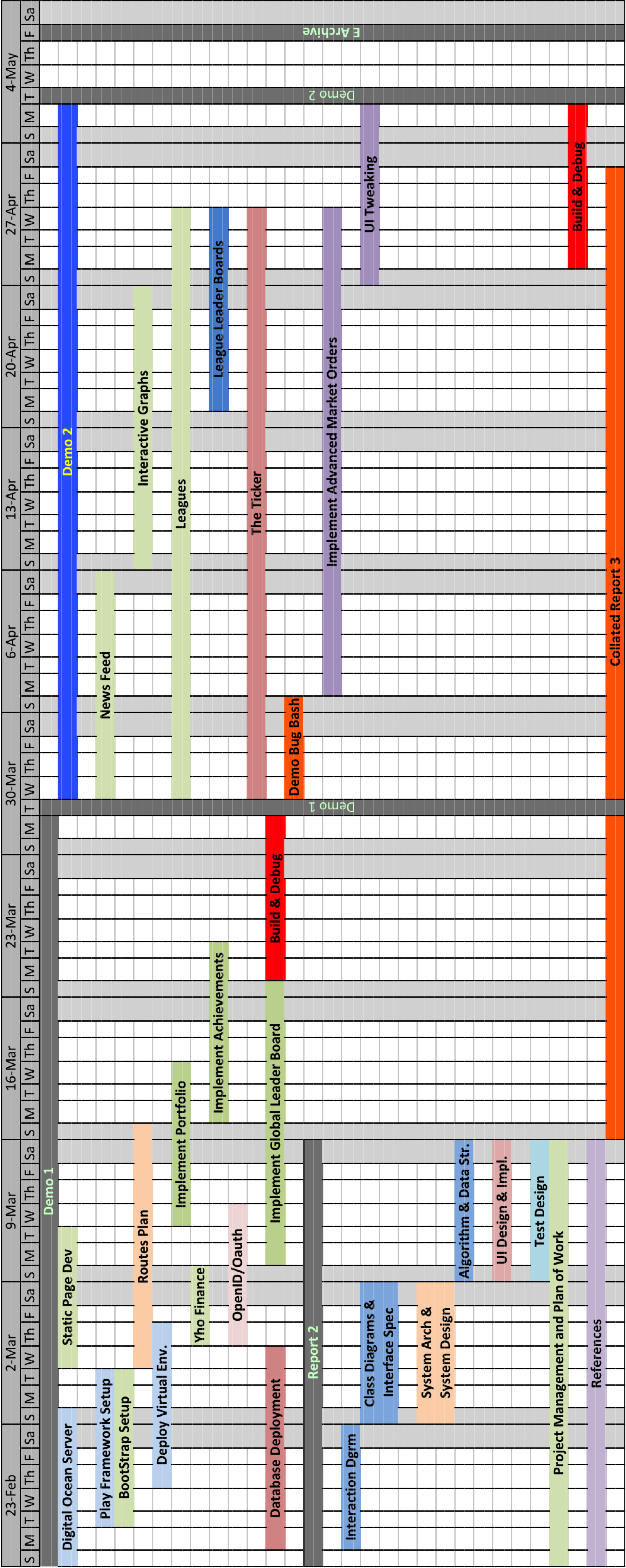
\includegraphics[height=9in]{./img/planOfWork.png}
\caption{This chart is the roadmap to meeting all our milestones.}
\end{figure}
